\chapter{Results}

Improved studies of several emission peaks of neutral Ba in SXe, which are first reported in the theses of B. Mong [ref] and S. Cook [ref], are reported.  The bleaching of several of these peaks is carefully observed ({\color{red}do a correction on p-meter sensitive area and on p-meter quantum efficiency, and also a spherical aberation correction for power??}), and a model of atomic transition rates is fit to this data.  Improved excitation spectra are achieved for all observed Ba emission peaks.  Images of $\leq$ 10\textsuperscript{3\textbf{?}} Ba atoms are achieved using the bleaching peaks.  Ultimately, images of Ba atoms at the few-atom level are achieved using the 619-nm fluorescence peak.  Improved studies of candidate fluorescence peaks of Ba\textsuperscript{+} in SXe are also reported.  

\section{Fluorescence of Ba in SXe}

The multiple peaks observed from deposits of Ba in SXe are attributed to Ba atoms occupying different Xe matrix sites, the phenomena of which are described in Chapter 3 {\color{red}(\emph{ref chap theory doesn't work})}.  Fig. [ref fig spectra for 10K, 50K, annealed 10K] shows spectra of Ba deposits under different conditions.  A deposit made at 11~K shows a different ... um how is this described in the paper?

excitspec of 50~K ... and 10~K?

leak rate dependence?

\section{Bleaching}

590 etc, model fit (see results intro paragraph)

\begin{figure}[H]
        \centering
                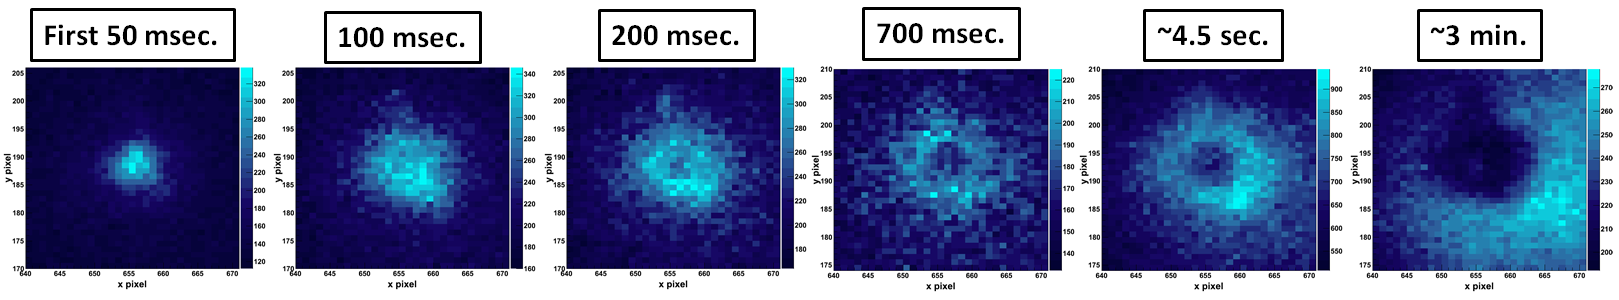
\includegraphics[width=.9\textwidth]{figures/hole_bleach_590.png}
                \caption{}
\label{fig:testfig}
\end{figure}

619, with the changes in time and I

\section{Imaging}

\subsection{Imaging 577- and 591-nm peaks}

\subsection{Imaging 619-nm peak}